\documentclass{standalone}
\usepackage{amsmath}
\usepackage{amsfonts}
\usepackage{tikz}
\usetikzlibrary{shapes.geometric}
\usetikzlibrary{arrows.meta}


\newcommand{\bt}{\mathbf{t}}
\newcommand{\bx}{\mathbf{x}}
\newcommand{\by}{\mathbf{y}}
\newcommand{\bz}{\mathbf{z}}
\newcommand{\eq}{=}


\begin{document}
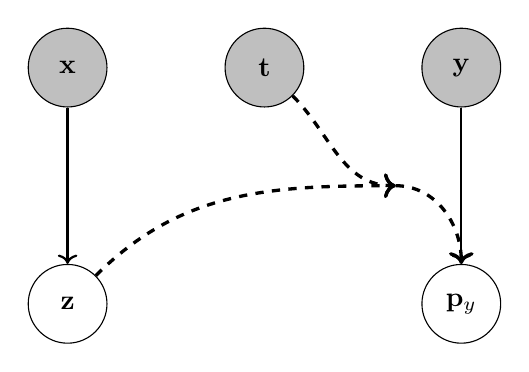
\begin{tikzpicture}
    \node[circle, draw=black, fill=lightgray, minimum size=1cm] (x) at (0, 3) {$\mathbf{x}$};
    \node[circle, draw=black, fill=lightgray, minimum size=1cm] (t) at (2.5, 3) {$\mathbf{t}$};
    \node[circle, draw=black, fill=lightgray, minimum size=1cm] (y) at (5, 3) {$\mathbf{y}$};
    \node[circle, draw=black, fill=white, minimum size=1cm] (z) at (0, 0) {$\mathbf{z}$};
    \node[circle, draw=black, fill=white, minimum size=1cm] (yprior) at (5, 0) {$\mathbf{p}_{y}$};
    
    \draw[->, thick] (x) to (z);
    \draw[->, dashed, very thick, out=45, in=180] (z) to node[below] {} (4.16666, 1.5);
    \draw[->, dashed, very thick, out=-45, in=180] (t) to node[below] {} (4.16666, 1.5);
    \draw[->, dashed, very thick, out=0, in=90] (4.16666, 1.5) to (yprior);
    \draw[->, thick, out=270, in=90] (y) to (yprior);
\end{tikzpicture}
\end{document}